%%% LaTeX Template
%%% This template is made for project reports
%%%	You may adjust it to your own needs/purposes
%%%
%%% Copyright: http://www.howtotex.com/
%%% Date: March 2011

%%% Preamble
\documentclass[paper=a4, fontsize=12pt]{scrartcl}	% Article class of KOMA-script with 11pt font and a4 format
\usepackage[T1]{fontenc}
\usepackage{fourier}
\usepackage[section]{placeins}
\usepackage{float}

\usepackage[english]{babel}															% English language/hyphenation
\usepackage[protrusion=true,expansion=true]{microtype}				% Better typography
\usepackage{amsmath,amsfonts,amsthm}										% Math packages
\usepackage[pdftex]{graphicx}														% Enable pdflatex
\usepackage{url}



%%% Custom sectioning (sectsty package)
\usepackage{sectsty}												% Custom sectioning (see below)
\allsectionsfont{\normalfont\scshape\textbf}	% Change font of al section commands

%%% Custom headers/footers (fancyhdr package)
\usepackage{fancyhdr}
\pagestyle{fancyplain}
\fancyhead{}														% No page header
\fancyfoot[L]{\small \url{Spring 2016}}		% You may remove/edit this line 
\fancyfoot[C]{}													% Empty
\fancyfoot[R]{\thepage}									% Pagenumbering
\renewcommand{\headrulewidth}{0pt}			% Remove header underlines
\renewcommand{\footrulewidth}{0pt}				% Remove footer underlines
\setlength{\headheight}{13.6pt}


%%% Equation and float numbering
\numberwithin{equation}{section}		% Equationnumbering: section.eq#
\numberwithin{figure}{section}			% Figurenumbering: section.fig#
\numberwithin{table}{section}				% Tablenumbering: section.tab#

%%% Maketitle metadata
\newcommand{\horrule}[1]{\rule{\linewidth}{#1}} 	% Horizontal rule

\title{
		%\vspace{-1in} 	
		\usefont{OT1}{bch}{b}{n}
		\normalfont \normalsize \textsc{\textbf{Department of Computer Science | University of Kentucky}} \\ [28pt]
		\horrule{0.5pt} \\[0.4cm]
		\huge Development of a Floodlight Application for Improving the Performance of GENI Experiments\\
		\horrule{2pt} \\[0.5cm]
		\normalfont \normalsize \textsc{\textbf{Masters project report}}
}
\author{
		\normalfont \normalsize \textsc{\textbf{Submitted By}} 
		\normalfont 								\normalsize
       	{: Sumaira Shamim}\\[-3pt]		\normalsize \\
       	\normalfont \normalsize \textsc{\textbf{Advisor}} 
       	\normalfont 								\normalsize
       	{: Dr. Zongming Fei}\\[-3pt]		\normalsize \\
  \today      
}
\date{}


%%% Begin document
\begin{document}
\maketitle
\thispagestyle{empty}

\newpage
\setcounter{page}{1}
%\section{Abstract}
%\newpage
\tableofcontents
\newpage

\section{Introduction}
The increasing advent of real time applications also bring the need of demanding Quality of Service guarantees and it is essential that the network protocols have the capability of meeting these requirements. The traditional networking is based on the best-effort principle and does not provide specific bandwidth, packet loss or latency guarantees for any application. Some efforts of traditional QoS architectures like DiffServ or IntServ require significant changes to the network design while Multiprotocol Label Switching (MPLS) lacks in ease of reconfiguration and adaptivity \cite{thesis}. The quality of service evaluation of a network is to make certain that the application receives its due set of connection parameters according to the QoS requirements of that application. The parameters can be throughput, End to end delay, Jitter (deviation from average end-to-end delay) and number of packets lost or damaged in the channel \cite{multipath}. 
\\
\\
The main goal of Software defined networks is to help create a smarter network then we have today. The concept of splitting the control plane and the data plane and increasing programmability of the network by taking the intelligence to a central controller allows us to make our networking entities more application aware.The advantages of a smarter network are better utilization of network resources, adaptability, lower cost and better services. Protocols such as OpenFlow can be used to establish this communication between the split control plane and the data plane and control the behavior of the entire network. The logically centralized control can help in defining distinct and complex network functions like load balancing and security based on the nature of the traffic or application \cite{thesis}. 
\\
\\
The decoupling of the control plane and data plane allows a high degree of control over flows that pass through the switches via intelligent controller applications using the northbound APIs for the controller. These applications can be leveraged for providing dynamic QoS guarantees for different classes of flows with different service requirements by making dynamic routing decisions or efficient priority queuing which is not possible in the traditional networks. For example flows belonging to an application with high QoS requirements can be diverted to a path with better bandwidth and less latency. Similarly, a flow belonging to a time-sensitive application can be placed in a priority queue of the OpenFlow switch.
\\
\\
This project focuses on research about how OpenFlow and Software Defined Networks can be used to provide Quality of Service. The project aims for setting up a GENI portal experiment for making routing path decisions based on available link bandwidth thereby improving the network performance. The project serves to be a proof of concept on how the behavior of individual network flows can be changed from the default shortest forwarding path in a GENI SDN experiment through Northbound API applications running on top of the SDN controller.
\\
\\
This report is organized as follows. Section 2 presents the literature review on related work for implementing QoS in software defined networks and summarizes the various techniques that are used. Section 3 presents a high level view of the experiment design and setup while Section 4 investigates in detail the implementation of the developed application. Section 5 demonstrates the experiment results and Section 6 discusses some of the challenges of the experiment. Section 7 and 8 describe the learning outcomes for this Master's project and conclude this report.

\section{Related work for implementing QoS in sdn}
This report summarizes the techniques that were researched for literature review on the project.

\subsection{Rate limiting and traffic shaping}
The rate limiting or traffic shaping technique is achieved by bandwidth control among the OpenvSwitch (OVS) ports for rate limiting. Standard OpenFlow protocol specifications like "enqueue" can be used for queuing traffic based on inspection of flows by the SDN controller in order to assign different queuing QoS policies for different flows. The queues inside OVS itself are configured by an administrator of OpenFlow versions less than 3.0 while versions 3.0 and above introduce "OF-Config" that will make this process much easier \cite{bigswitch}. 
\\
\\
Since only bandwidth guaratees and FIFO scheduling is not enough to provide QoS guarantees in SDN, using multiple packet schedulers of Linux kernel e.g., Hierarchical Token Bucket, Randonly Early detection and Stochastic Fairness queuing can be utilized to overcome packet scheduling issues. The strong traffic control system of Linux can be used to provide traffic shaping, queuing and congestion avoidance. This approach would require data path extensions for OpenFlow for kernel space queues \cite{scheduler}.
\\
\\
Some QoS extensions to OpenFlow have been developed in \cite{convergence} that have the capability of taking in high level QoS requirements of applications and automatically modify the QoS parameters on network devices in the form of rate limiters and dynamic priority assignment. This controller removes the need of manually configuring QoS requirements for each device in the network and centrally controls these configurations. 
\subsection{Differentiated Services Code Point (DSCP)}
This technique is established by using the 8 Type of Service bits in existing IP header for implementing differentiating class of service. Standard OpenFlow protocol specifications allow rewriting of the Type of Service field in the IP header using "network ToS". This is achieved by the SDN controller after flow matching and classification according to different ToS polices for different flows \cite{bigswitch}.
\subsection{Multipath routing}
The idea of multipath routing is to split and balance a flow among a set of alternative paths using a Multipath agent which splits tcp session into multiple virtual sessions at the end host by starting internal sockets. The controller can intercept the first packet of each new connection and find out the application it belongs to by inspecting the payload and make sure the flows with the same connection take different paths. All the flows are multiplexed together via a multiflow agent at the destination host. A speciating routing module in the controller keeps track of the subflows, QoS policies and dynamic calculation of paths which serve the best QoS to the flows \cite{multipath}.
\subsection{Dynamic routing of specific flows}
This approach is designed for special QoS flows like multimedia flows where timely delivery is preferred over reliability usually without affecting other types of traffic. The QoS flows can be dynamically routed on different paths while the rest of the data flows remain on the shortest optimal path for them. The traffic can be differentiated by Traffic class header field in MPLS, TOS (Type of Service) field of IPv4 header, Traffic class field in IPv6 header, source IP address of a known multimedia server and TCP port numbers. Collection of current global network state information like delay, bandwidth and rate of packet loss is also required for dynamic routing \cite{openqos}.
\\
\\
Another approach for dynamic routing is by using two level QoS flows for multimedia like MPEG-4 which encodes videos in a base layer and enhancement layers. The controller identifies the level 1 QoS (base layer), level 2 QoS (enhancement layers) and normal traffic flows and updates the switches with calculated dynamic routes for level 1 QoS and level 2 QoS flows after estimating bandwidth and delays on the links \cite{video}.
\\
\\
Another technique in \cite{thesis} tries to find an optimal path between two end points with the minimum cost (that does not increase the capacity of any link) after ruling out the links that break specified QoS constraints.(i-e delay and packet loss do not increase a threshold).The architecture dynamically updates the network parameters to become aware of the status of the network and calculate the best route according to the QoS specified policies. The model is based on "multi-commodity flow constrained shortest path problem (MCFSP)" .

\section{Project Design}
\subsection{Experiment Setup}
The experiment is set up in GENI portal using Xen virtual machines as hosts and Open vSwitch nodes as virtual switches between them. The switches are configured with default shortest path routing rules for each of the hosts using an SDN controller. The SDN controller used is Floodlight open source controller which exposes a REST API for the northbound applications to use. The northbound QoS application for the experiment is developed in Python. It uses python packages like Networkx\footnote{https://networkx.github.io\label{networkx}} and untangle\footnote{https://untangle.readthedocs.org\label{untangle}} in order to construct the topology using the information provided by the controller REST API and RSpec document provided by the GENI portal. 
\subsection{The network topology}
The topology constructed in GENI portal is shown in Figure \ref{Fig 3.1}. The topology is not linear and has multiple paths between a pair of hosts in order to have alternate paths for routing flows based on bandwidth. The nodes labeled as switches run Openvswitch on them configured to use an OVS bridge to connect to the hosts and other OVS nodes.
\\
\\
Each of the OpenFlow switches (OVS) have a Datapath id (DPID) associated with them which is used by the SDN controller to identify and control the switches. Using the web interface of the Floodlight controller, we can see the switches connected to the controller and the various information statistics related to them in Figure \ref{Fig 3.2}.
\begin{figure}[H]
\begin{center}
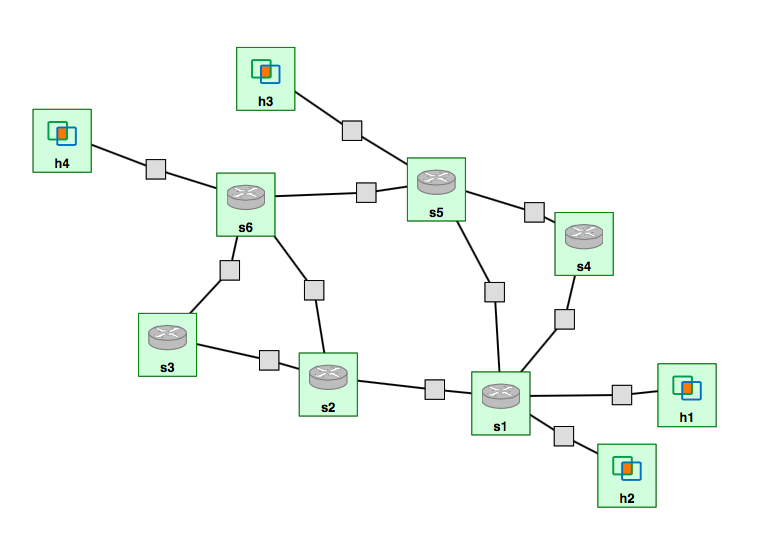
\includegraphics[scale=0.55]{topology.png}   
\end{center}
 \caption{GENI topology}
 \label{Fig 3.1}
\end{figure}
\begin{figure}[H]
\begin{center}
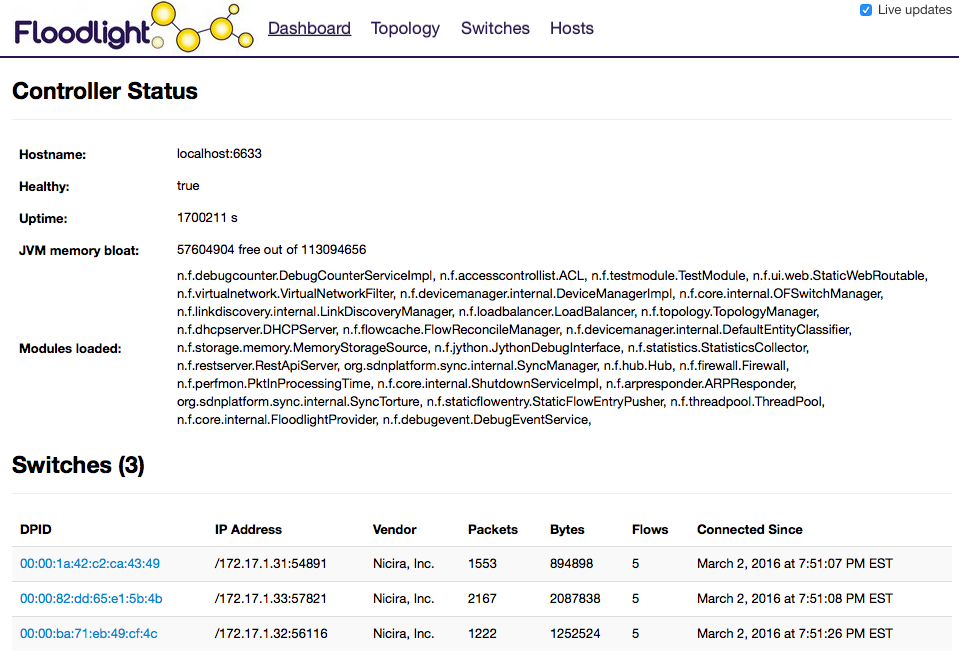
\includegraphics[scale=0.55]{floodlight.png}   
\end{center}
 \caption{Floodlight dashboard}
 \label{Fig 3.2}
\end{figure}
We can also see the OpenFlow rules that a switch is configured with in Figure \ref{Fig 3.3}. Right now, the rules shown are default shortest path rules with OpenFlow priority `1' that the floodlight controller pushed into the switches using the static flow pusher REST API.
\begin{figure}[H]
\begin{center}
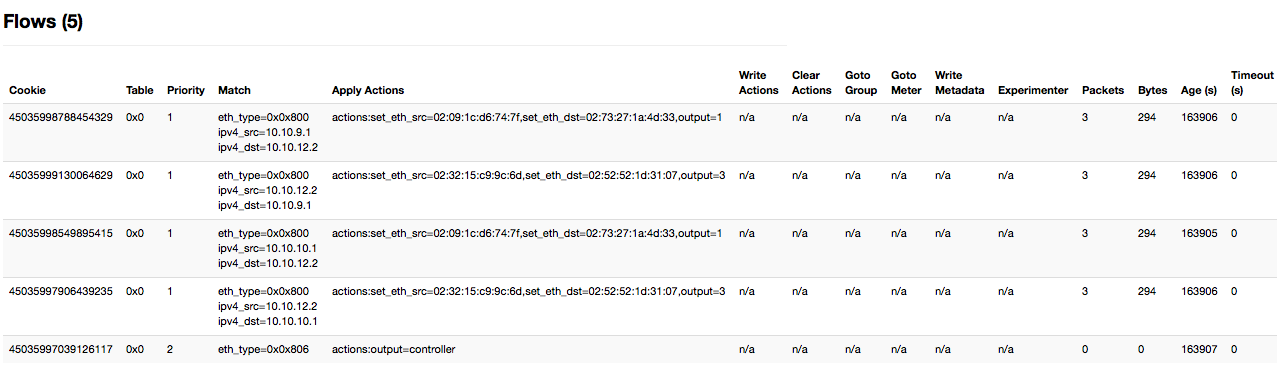
\includegraphics[scale=0.35]{rules.png}   
\end{center}
 \caption{Rule table in OpenFlow switch}
 \label{Fig 3.3}
\end{figure}
\subsection{Control Flow}
The control flow of the application starts from constructing the network graph, polling the OpenFlow switches using the floodlight REST API to find active flows and then uses the statistics collector module of floodlight to query link statistics. Based on the statistics received, the application chooses a different path for an active flow based on available link bandwidth and available paths. The application control flow is shown in Figure \ref{Flow}.
\begin{figure}
\begin{center}
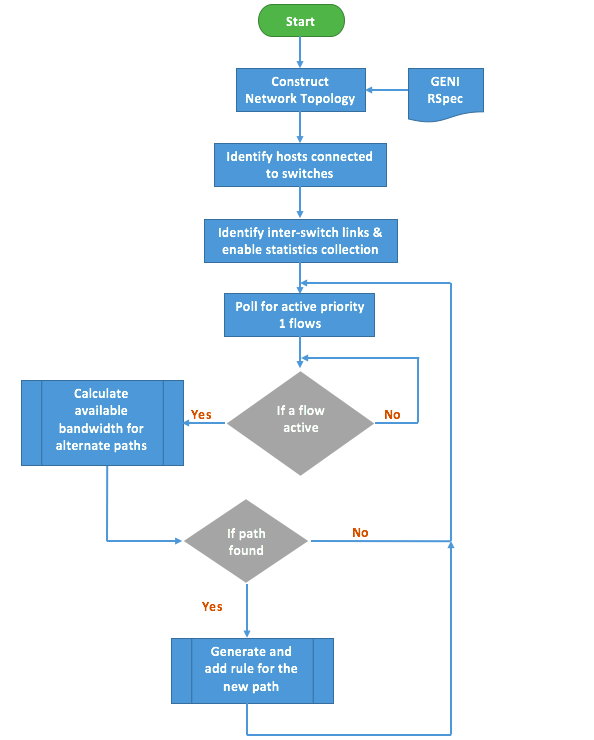
\includegraphics[scale=0.65]{flowchart.png}   
\end{center}
 \caption{Control Flow of the application}
 \label{Flow}
\end{figure}

\subsection{Design Decisions}
The design decisions taken are the following:
\begin{itemize}
\item The topology is constructed using Python Networkx\footref{networkx} library undirected graph. The information for the nodes and the edges is received from the GENI RSpec document as well as the Floodlight controller REST API calls.
\item The inter-switch links have been assigned a total bandwidth of 50 Mbps each and the switch-hosts links have the default bandwidth of 100 Mbps as configured by GENI portal.
\item As a default setting of the statistics collector module of Floodlight controller, the links are polled every 10 seconds for updated information. No settings of the module have been changed in this experiment.
\item The different simple paths are only on an end-to-end basis for a pair of hosts. A simple path means that no node is repeated in a path between two hosts.
\item A switch can only decide to change the shortest default path for a flow if the sender's IP is on the same subnet as the switch's interface.
\item The active flows with priority `1' are decided by polling the switches every 10 seconds and comparing the last packets hit count with the new polled information.
\item The application selects a different path based on aggregate available bandwidth from a list of unshared / unused simple paths between the source and the destination.
\item The application tries to select the next available shortest path between the source and destination whose available bandwidth is greater or equal to atleast 95\% of another alternate longer path.
\item The aggregate available bandwidth for a path is actually the minimum available link bandwidth on the set of inter-switch links on that path.
\item If a better path is not available, the flow is kept on the shortest default path.
\item The QoS rule written by the controller in the switches for a particular flow has an OpenFlow priority of `3' which makes sure that it receives precedence to any default shortest path rules for the same flow with priority `1'. Once a different path is selected for a flow, it is not changed again until the application quits.

\end{itemize}
\section{Project Implementation}
This section goes over the steps of the developed application summarized in Figure \ref{Flow} in detail.
\subsection{Constructing the topology}
The application reads in the RSpec XML document from GENI portal and parses information about the names and interfaces of the nodes. The Python library used for parsing is "untangle\footref{untangle}" which converts XML to python objects. The node data items consist of the IP address, MAC address and port number for each of the interfaces connected to that node. The application then queries the controller using REST API commands to get respective OpenFlow Datapath ids (DPIDs) for the switches in the topology. Following command is used to get the DPID list from the controller:
\textit{
\begin{center}
"curl -s http://<controllerIp>/wm/core/controller/switches/json" 
\end{center}
}
To match a DPID received from the controller to the node name in GENI, the following REST API command is used:
\textit{
\begin{center}
"curl -s http://<controllerIp>/wm/core/switch/all/desc/json"
\end{center}
}
This command returns features of all the switches and the field 'datapathDescription' gives information to match the DPID to the node name from GENI.Similarly, the RSpec does not give information about the switch ports for the interfaces and the information about port numbers has to be queried from the controller using the following command:
\textit{
\begin{center}
"curl -s http://<controllerIp>/wm/core/switch/all/features/json"
\end{center}
}
For constructing the network graph after parsing the RSpec and querying the controller for the desired information, Python library "Networkx\footref{networkx}" is used which provides data structures for constructing network graphs. The library creates a Network object to which nodes and edges can be added. The nodes have the data items for interfaces as described above as well as the DPID and port numbers matched to the nodes using the controller information. 
\\
\\
Since the RSpec document or the controller do not provide information about the neighbors of the nodes or which interface is connected to which neighbor, the inter-host links are identified by matching the respective IP addresses in order to construct the edges between the nodes for the graph.

\subsection{Identifying hosts connected to the switches}
As mentioned in the design decisions, A switch can only decide to change the path for a flow if the sender's IP is on the same subnet as the switch's interface. To implement this, a structure 'switchHostsFlows' is constructed which specifies which hosts are on the switch subnet and which are the interfaces that connect to another switch instead of a host. It also specifies the possible source and destination pairs of a switch's traffic after polling all the shortest path flows in the OpenFlow table of that switch. This structure also maintains the flow statistics for each pair of source and destination hosts in the form of the last packet count. This information is later used to determine active flows in the network.
\\
\\
The hosts connected to the switch are identified by comparing the network address of interfaces of the hosts to the /24 network prefix of the interfaces of the particular switch. This structure only references the nodes which play the role of "hosts" on the network and not the ones which play the role of "switches".

\subsection{Enabling statistics collection}
In order to take advantage of the Floodlight controller statistics module REST API, it needs to be enabled in all the OpenFlow switches in the network. The command used to enable the statistics collection in the application is:
\textit{
\begin{center}
"curl -X POST -d ` ' http://< controllerIp>/wm/statistics/config/enable/json"
\end{center}
}
After statistics are enabled in the switches, the application can query the controller using the REST API commands specifying the switch using OpenFlow DPID and the desired port using the following command:
\textit{
\begin{center}
"curl http://<controllerIp>/wm/statistics/bandwidth/<switchDPID>/<port>/json"
\end{center}
}
The reply to the above command returns the transmission and reception bandwidth per switch per port in bits per second. The default interval when the bandwidth is reassessed by the controller is every 10 seconds \cite{stats}.
\subsection{Identifying inter-switch links}
The application also creates a list of links between the switches and the respective output switch ports for those links called the "interswitchLinks". This is important because the bandwidth calculation for paths is done solely on the basis of available bandwidth on the switch-switch links and not the switch-host links.
\subsection{Determine active flows}
As described in section 4.3.2, the structure "switchHostsFlows" keeps track of the last known packet count for a particular flow from a host to a destination. The application queries the controller to poll the switches for a list of flow statistics every 10 seconds using the command:
\textit{
\begin{center}
"curl -s http://<controllerIp>/wm/core/switch/<switchDPID>/flow/json" 
\end{center}
}
For each shortest default path flow rule returned, the application checks if the source IP is from the same subnet as an interface from the switch DPID being polled by comparing to the list of switch hosts in 'switchHostsFlows'. If determined to be the gateway switch for that flow, the new packet count is compared to the stored last known packet count to determine if the flow is active. If a shortest default path flow rule is found active, the function to calculate bandwidth for all alternate paths is called.

\subsection{Calculate available bandwidth for alternate paths}
The "calculate bandwidth for paths function" receives two arguments; a source and a target for an active flow on its default shortest path. The function calculates all simple paths between the source and the target using "all\_simple\_paths" method of the Python Networkx\footref{networkx} library. A simple path means that no node is repeated in a path between two hosts. If there is only one simple path returned, no alternate path is present between the two hosts i.e. only the shortest default path is available and the program returns to polling other active shortest default path flows. Figure \ref{pseudo} shows the pseudocode for this function.
\\
\\
Using the information from the "interswitchLinks", the function uses the curl command from section 4.3.3 to get the transmission (TX) and reception bandwidth (RX) per switch per inter-switch port in bits per second. The TX and RX values are added to find the bandwidth usage in bits per second and then subtracted from the actual known link bandwidth to get available link bandwidth for each switch port and stored in a structure for using in path selection.

\paragraph{Global QoS rules structure}
In order to keep track of all the QoS flows of priority `3' added in the topology, a global list "QoSFlowsList" is maintained. This structure has 4 fields per rule entry; a source, a target, the complete path and the inter-switch links involved. This structure aids in the decision of selecting an unused / unshared path between different nodes in order to achieve maximum throughput when competing traffic is targeted from different sources to the same destination. The function also checks this list to ensure that a QoS flow for a source and destination pair does not already exist. The major functions of this list are:
\begin{itemize}
\item If the list is empty at the time application detects the very first active flow, the shortest default path is added as a QoS rule for that flow since all the links have the same available bandwidth. This path is stored in the global list so no other flow will be assigned this path.
\item The second purpose is to check if a rule already exists in the global list for a flow so that there is no need to make further path changes for a flow.
\item The third role of the list is to check if for a given source-target, a reverse path "target-source" exists in the list. If yes, then the reverse path is added to the list and also sent to the rule generation function.
\item The final purpose of this list is to find best possible unused or unshared inter-switch link paths for each incoming active flow based on length of path and aggregate available bandwidth.
\end{itemize}
\begin{figure}[H]
\begin{center}
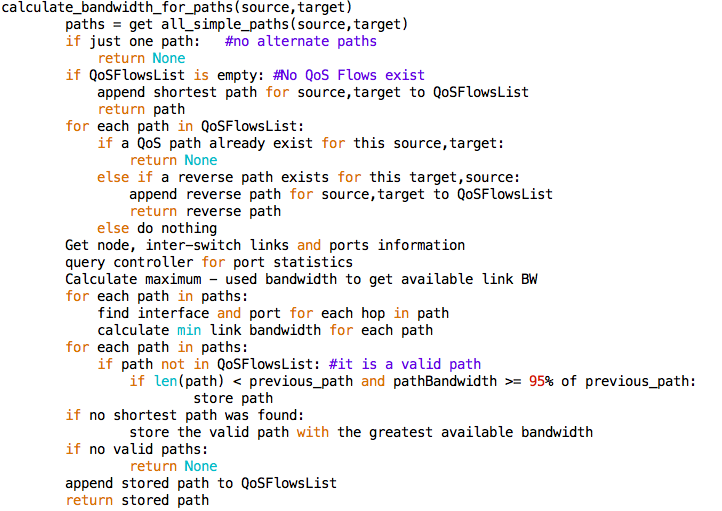
\includegraphics[scale=0.55]{pseudo.png}   
\end{center}
 \caption{Pseudocode for calculate\_bandwidth\_for\_paths}
 \label{pseudo}
\end{figure}
For each simple path calculated for a source-target pair, the function decides which switches and inter-switch ports are involved on that path. Using the stored bandwidth statistics, it calculates the available bandwidth for each path by finding the minimum available bandwidth for a link involved in that path.
\\
\\
After calculating available bandwidths on all paths, the function checks if the paths are valid unused or unshared paths by checking the global QoS flows list. Then the function checks if any of the bandwidth values of the valid paths are better than the default shortest path. If yes, then it chooses the next shortest path with the best available value, adds it to QoS flows list and returns the path. If not, then the function returns none since there is no path available that will guarantee good bandwidth without compromising other competing traffic and the flow remains on shortest path.

\subsection{Generate rule for path}
The "generate rule for path" function is called if the "calculate bandwidth for paths function" returns an alternate path for a pair of hosts. The function takes in three arguments; a path which is returned by the bandwidth function, a source IP and a destination IP. The function first checks the OpenFlow rule table of the switches involved in that path for a match of a priority `3' rule for the same source and destination IP using the following command.
\textit{
\begin{center}
"curl -s http://<controllerIp>/wm/staticflowpusher/list/<switchDPID>/json" 
\end{center}
}
If a rule already exists, the function returns and does not generate a new priority `3' rule. If no rule exists, the function determines the node and the next hop interface for each node in the path, finds the MAC address and switch port for forwarding and constructs a flow rule in JSON format to send via the static flow pusher REST API of Floodlight controller. A sample flow rule is shown in Figure \ref{sample}. The command used by the application to push a generated flow through the controller to the switch is:
\textit{
\begin{center}
"curl -X POST -d `"+<JSON\_rule>+"' http://<controllerIp>/wm/staticflowpusher/json" 
\end{center}
}
\begin{figure}[H]
\begin{center}
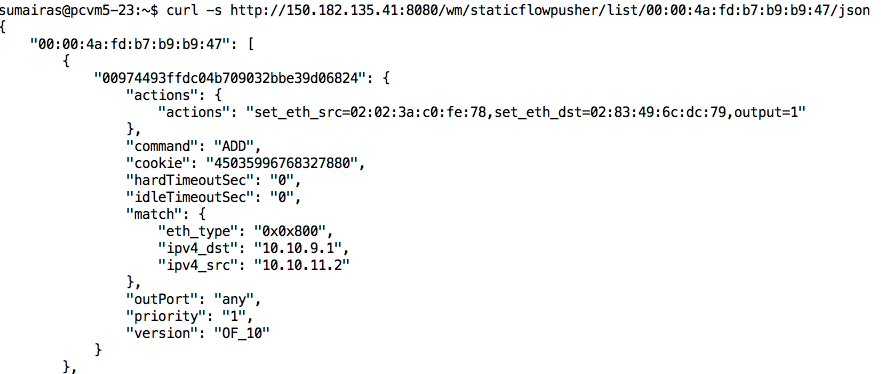
\includegraphics[scale=0.4]{flow.png}   
\end{center}
 \caption{A sample flow}
 \label{sample}
\end{figure}
\subsection{Deletion of QoS Flows}
If the application is aborted throught the command prompt, we need to delete all the QoS flows so that new QoS rules can be set up the next time application is started. In order to delete any rule inserted using the static flow pusher API of Floodlight, the globally unique flow rule name needs to be tracked. In Section 4.7, if any rule is pushed using the static flow pusher, the globally unique flow name is stored in a list "toDelete". When the signal to quit application is sent through the keyboard, the function delete\_rules is called which deletes all the static rules in the switches using the following REST API command and exits the application.
\textit{
\begin{center}
"curl -X DELETE -d '{name:<flow name>}' http:// controllerIp/wm/staticflowpusher/json"
\end{center}
}

\subsection{Application Testing}
The scenarios for testing the performance of the application are listed below:
\subsubsection{File parsing for topology construction}
In case of an absent or corrupted GENI RSpec file for topology construction, the application catches the error and exits with a "File error" message. The XML file parsing implementing using Python untangle\footref{untangle} library logic and function calls for constructing the network graph nodes are placed in a "try" block. Any exception is caught and application is properly exited. This prevents the errors in topology construction to be carried forward into the link identification and creation of other structures.
\subsubsection{Calculate bandwidth for paths function}
There are multiple checks to ensure the calculate bandwidth for paths function does not cause errors in the application which are described below:
\begin{itemize}
\item The function is passed no user input and only the source and target of an active flow polled from the controller are passed as arguments.
\item If the source and target passed as arguments have no alternate paths, the function returns "None" and the control passes to polling active flows without errors.
\item Since each QoS Flow is added to the global QoS list before pushed into the switches by the controller, the function always checks if a QoS flow for the passed arguments already exists. If yes, then a "None" is returned.
\item The function also checks if a reverse path for the source and target arguments exists in the QoS list. This prevents generation of an entirely different reverse path for a source and target. 
\item Before choosing an alternate path, the function always checks if that path is a valid and unused one by checking the QoS list to prevent using a path already assigned.
\item If no better path was found, the function will return "None" and the control will pass to polling active flows again.
\end{itemize}

\subsubsection{Rule generation function}
The rule generation function is only called when the calculate bandwidth function returns a valid path. Since no other input is received by the rule generation function, in case of a valid path argument the function generates and passes the rules to the controller with no errors.

\section{Results}
\subsection{Traffic from host 1 and host 2 to host 3}
To test the effectiveness of the applicaton, we need to test throughput achieved with competing traffic with and without the application running. We will test this by sending traffic from host 1 (h1) to host 3 (h3) and host 2 (h2) to host 3 (h3) at the same time. Figure \ref{Shorth3} shows the shortest path setup from h1-h3 and h2-h3 without the application running.
\begin{figure}[H]
\begin{center}
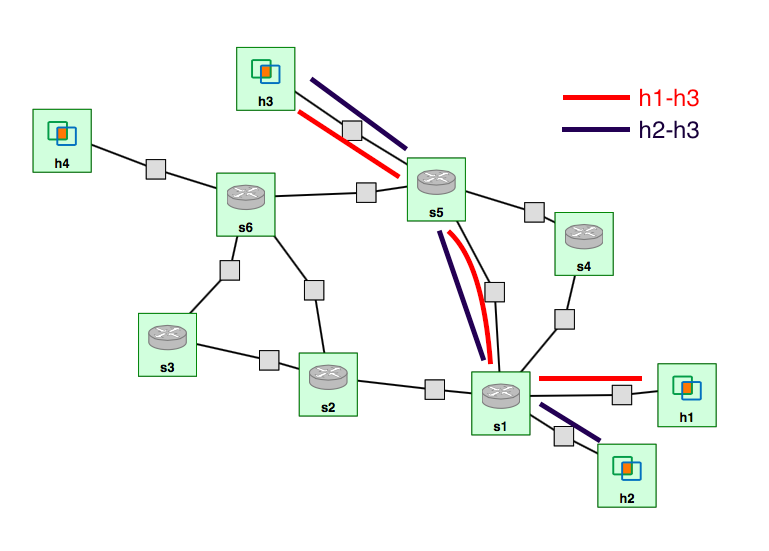
\includegraphics[scale=0.45]{shortest.png}   
\end{center}
 \caption{Shortest paths from h1,h2 to h3}
 \label{Shorth3}
\end{figure}

After running the application, we run "iperf" from h1 to h3 and since this is the first active flow, the shortest path is added as a QoS flow for h1-h3 and also a reverse path for h3-h1 as shown in Figure \ref{Outh1h3}. Next, we run "iperf"  from h2 to h3. The application discovers the active flow, queries for link bandwidth and chooses the next shortest and unused path with the better bandwidth for h2-h3 as shown in Figure \ref{Outh2h3}.
\begin{figure}[H]
\begin{center}
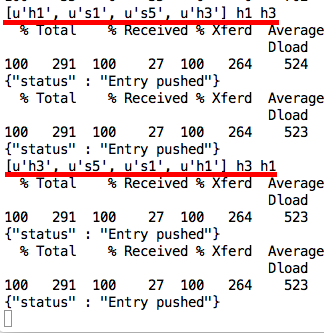
\includegraphics[scale=0.45]{h1-h3.png}   
\end{center}
 \caption{Application output for QoS Flow from h1-h3 and h3-h1}
 \label{Outh1h3}
\end{figure}
\begin{figure}[H]
\begin{center}
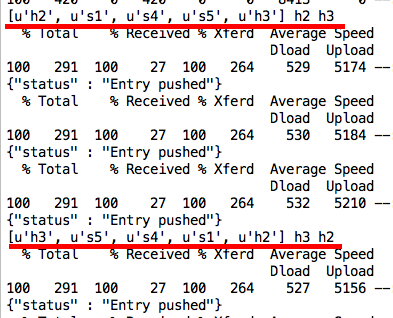
\includegraphics[scale=0.45]{h2-h3.png}   
\end{center}
 \caption{Application output for QoS Flow from h2-h3 and h3-h2}
 \label{Outh2h3}
\end{figure}
Figure \ref{Qosh3} shows the final set up for the paths for h1-h3 and h2-h3 with the application running.
\begin{figure}[H]
\begin{center}
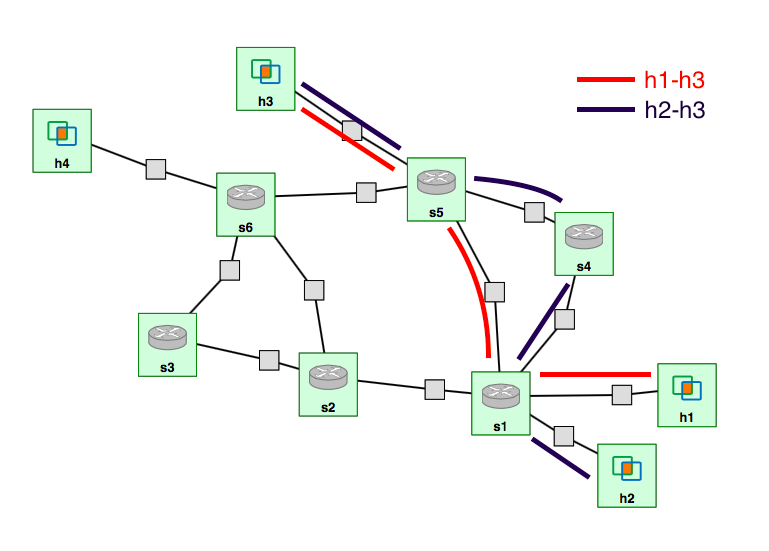
\includegraphics[scale=0.45]{qos.png}   
\end{center}
 \caption{New QoS paths from h1,h2 to h3}
 \label{Qosh3}
\end{figure}

To test the throughput, we will "iperf" from h1-h3 and h2-h3 at the same time. The maximum link bandwidth that can be achieved is 50 Mbps. Figure \ref{h123WO} shows the results achieved without the QoS application running and Figure \ref{h123W} shows the results achieved with the QoS application running using the paths shows in \ref{Qosh3}. 
\begin{figure}[H]
\begin{center}
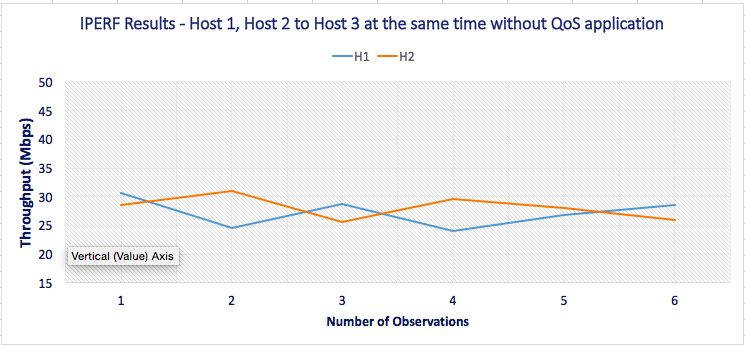
\includegraphics[scale=0.45]{h123WO.png}   
\end{center}
 \caption{Iperf results from h1,h2 to h3 without application}
 \label{h123WO}
\end{figure}
\begin{figure}[H]
\begin{center}
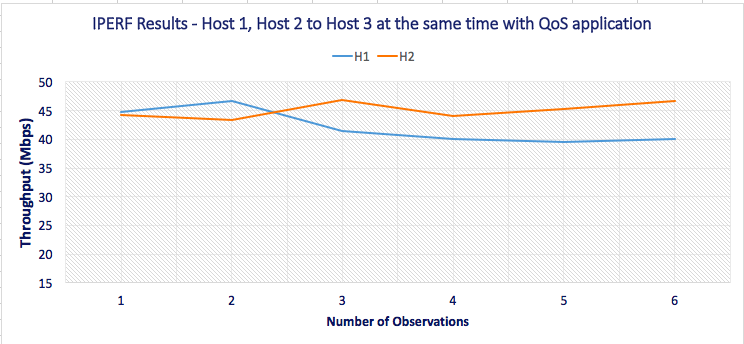
\includegraphics[scale=0.45]{h123W.png}   
\end{center}
 \caption{Iperf results from h1,h2 to h3 with application}
 \label{h123W}
\end{figure}
It is clear that the QoS application paths achieve near link bandwidth in case of competing traffic targeted at the same destination.
\subsection{Traffic from host 1 and host 2 to host 4}
Similarly, we test the throughtput achieved when we send traffic from host 1 (h1) and host 2 (h2) to host 4 (h4) at the same time. At this time, QoS paths have been set up for h1-h3 and h2-h3 and the application is running. Figure \ref{Shorth4} shows the shortest default paths for h1-h4 and h2-h4.
\begin{figure}[H]
\begin{center}
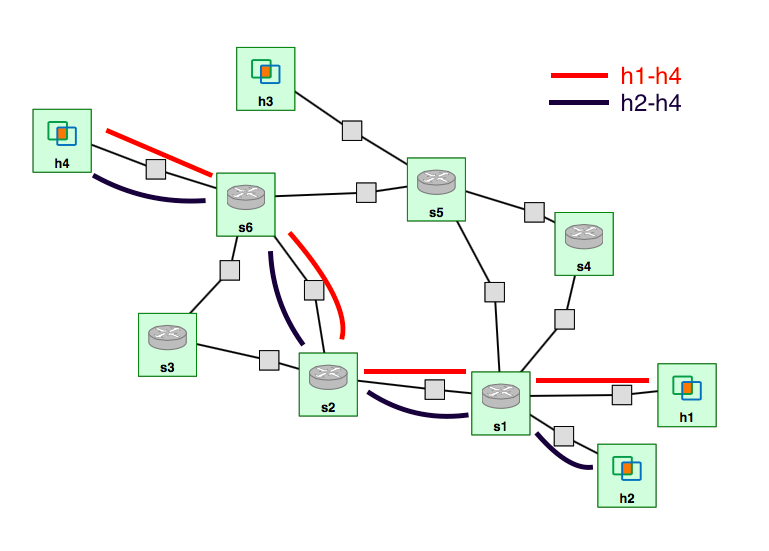
\includegraphics[scale=0.45]{shortesth4.png}   
\end{center}
 \caption{Shortest paths from h1,h2 to h4}
 \label{Shorth4}
\end{figure}
Now, we run "iperf" from h1 to h4 and the next shortest and unused path with the better available bandwidth is added as a QoS flow for h1-h4 and also a reverse path for h4-h1 as shown in Figure \ref{Outh1h4}. Next, we run "iperf"  from h2 to h4. The application discovers the active flow, queries for link bandwidth and chooses the next shortest and unused path with the better bandwidth for h2-h4 as shown in Figure \ref{Outh2h4}.

\begin{figure}[H]
\begin{center}
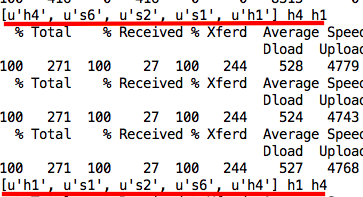
\includegraphics[scale=0.45]{h1-h4.png}   
\end{center}
 \caption{Application output for QoS Flow from h1-h4 and h4-h1}
 \label{Outh1h4}
\end{figure}

\begin{figure}[H]
\begin{center}
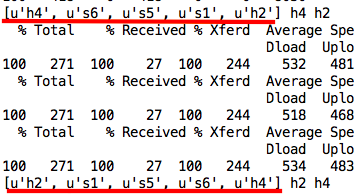
\includegraphics[scale=0.45]{h2-h4.png}   
\end{center}
 \caption{Application output for QoS Flow from h2-h4 and h4-h2}
 \label{Outh2h4}
\end{figure}

Figure \ref{Qosh4} shows the final set up for the paths for h1-h4 and h2-h4 with the application running.
\begin{figure}[H]
\begin{center}
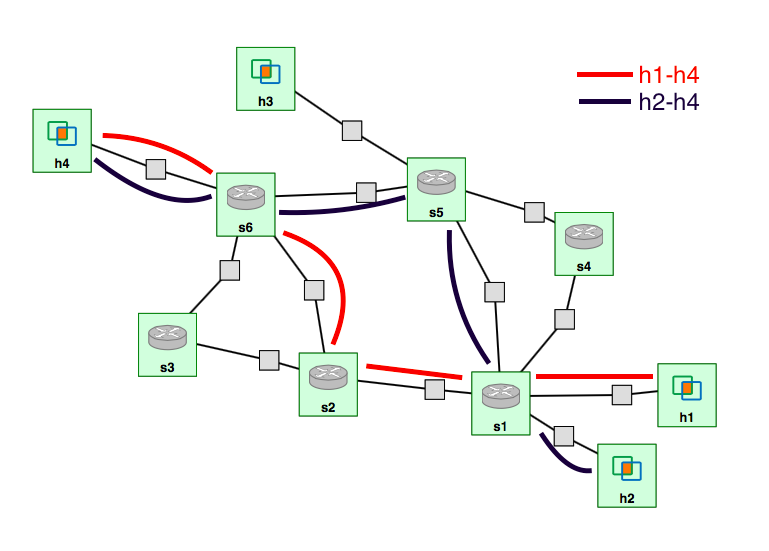
\includegraphics[scale=0.45]{qosh4.png}   
\end{center}
 \caption{New QoS paths from h1,h2 to h4}
 \label{Qosh4}
\end{figure}

To test the throughput, we will "iperf" from h1-h4 and h2-h4 at the same time. The maximum link bandwidth that can be achieved is 50 Mbps. Figure \ref{h124WO} shows the results achieved without the QoS application running and Figure \ref{h124W} shows the results achieved with the QoS application running using the paths shows in \ref{Qosh4}. 
\begin{figure}[H]
\begin{center}
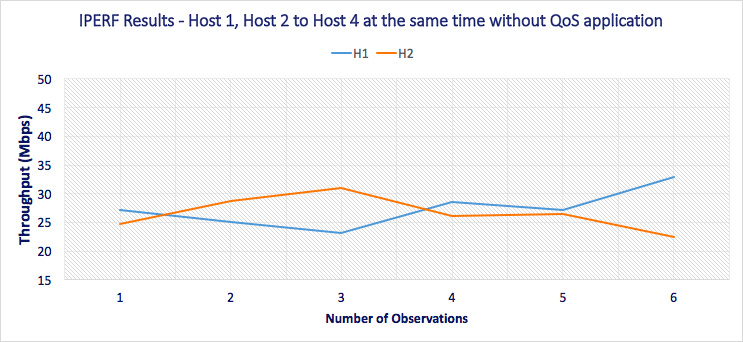
\includegraphics[scale=0.45]{h124WO.png}   
\end{center}
 \caption{Iperf results from h1,h2 to h4 without application}
 \label{h124WO}
\end{figure}
\begin{figure}[H]
\begin{center}
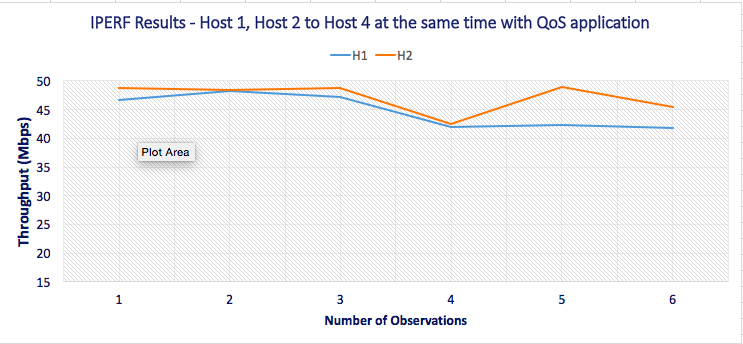
\includegraphics[scale=0.45]{h124W.png}   
\end{center}
 \caption{Iperf results from h1,h2 to h4 with application}
 \label{h124W}
\end{figure}
It is clear that the QoS application paths achieve much better link bandwidth in case of competing traffic targeted at the same destination.
\section{Challenges}
There were a few challenges that were faced during the experiment setup.
\subsection{Default L2 learning switch}
The default modules of Floodlight controller do not have the capability to perform shortest path routing between hosts on different subnets. There is no ARP module that will take care of the ARP requests if we use a simple layer 2 learning switch module in the controller. Therefore, some advanced features of GENI Desktop were used to initialize all the OVS nodes with shortest path rules that modify the Ethernet header after sending all the ARP traffic to the controller. This also requires that the QoS Flow rule action field built by the application must contain clauses which modify the Ethernet header with source and destination MAC address at each hop for each source-destination host IP pair.
\subsection{Bandwidth design decision}
There is also a design decision involved which is the time interval at which the controller statistics module reassesses the bandwidth at the links. The default time used by the controller is 10 seconds and the application uses the default setting. According to Floodlight, the statistics provide a ballpark figure. OpenFlow does not provide any statistics which have the notion of time and the controller needs to calculate bandwidth using raw byte counters at two instances in time and return the value if requested using the statistics module. The 10 second time serves as a tradeoff between getting less error prone bandwidth calculation (to make control plane latency insignificant) and overburdening the switches with statistics requests by the controller to get real time bandwidth \cite{stats}.
\subsection{Dynamic path changing}
The initial experiment setup changed the path for each flow dynamically based on link bandwidth every 10 seconds if a better path was available. This was not scalable since changing the path continuously does incur overhead at both the northbound and southbound interfaces. Also, it mirrored the same problem since the beginning of internet that all flows tend to choose the same better path with greater bandwidth at one instance in time which congests that path and leaves the other alternate paths with more capacity but unused. Since the bandwidth stats are reassessed by the controller every 10 seconds, even if we query the stats every time when a flow is active does not guarantee that the seemingly best path in terms of bandwidth was not assigned to another flow in the same 10 second time period.

\section{Learning Outcomes}
The learning outcomes from this project were the following:
\begin{itemize}
\item Knowledge of different techniques and methods utilized for improving quality of service in software defined networks.
\item Configuring an OpenFlow topology in GENI portal and initializing and configuring OpenvSwitch nodes to set up OVS bridges for networking.
\item Connecting an SDN controller "Floodlight" with the configured OVS nodes and using the controller's REST API to interact with the OpenFlow switches.
\item Developing a python application to parse information from GENI portal and the controller to construct the topology and change the default behavior of the network for improving performance.
\item Discovering challenges with real time bandwidth information and decision making for dynamic routing.
\end{itemize}

\section{Conclusion}
This project serves to be a proof of concept of how we can use intelligent controller applications to change the default behavior of a GENI network. For dynamic routing based on bandwidth, more work needs to be done to tackle the challenges mentioned in Section 6. Maybe if OpenFlow protocols introduces some standards for adding byte counters with time notion, the overhead and latency incurred at the controller for calculating bandwidth by keeping track of byte counters at two time instances can be avoided and more real time statistics can be sent through the REST API to applications.
\\
\\
This experiment fixes a path for different flows as they arrive if a better bandwidth path can be provided to them. This concept can be used to target better service for a higher class of flows either coming from a priority server distinguished by the server IP address, Multiprotocol Label Switching (MPLS) traffic or multimedia traffic from a known server while other flows can remain on the shortest best effort paths. It is shown in the results that the throughput achieved by using the application was almost at the link capacity when competing traffic was targeted to the same destination as compared to ~50\% of link capacity achieved by just shortest path.

\bibliographystyle{ieeetr}% Select the citation style e.g. ieeetr
\bibliography{Smartgrid}% write the directory to the .bib file
%%% End document

\end{document}